\section{Zielsetzung}
Mit dem Franck-Hertz-Versuch soll die Quantennatur der Elektronenhülle,
wie sie durch das Bohrsche Atommodell, aber auch in der modernen Quantenmechanik,
postuliert wird, bestätigt werden. Dies soll dadurch gezeigt werden, dass Elektronen
in einem Gas beschleunigt werden. Wenn sich bei bestimmten Beschleunigungsspannungen die Zahl
ankommender Elektronen an der Anode abrupt deutlich reduziert, kann davon ausgegangen werden, dass das Gas erst bei einer diskreten 
Energie der Elektronen angeregt werden kann. Damit wäre gezeigt, dass Atome Energie nur 
quantisiert absorbieren können. Da ein angeregtes Atom nach einer kurzen Zeit in den Grundzustand
zurückfällt, emittiert das Quecksilber Photonen mit der gleichen Energiedifferenz, die es absorbiert hat.
Die entsprechende Wellenlänge soll in diesem Versuch ebenfalls ermittelt werden. Dafür muss das Kontaktpotential 
ermittelt werden und Frank-Hertz Kurven aufgenommen werden.
\section{Theorie}
\label{sec:Theorie}
Der Franck-Hertz-Versuch ist ein sogenannter Elektronenstoßexperiment. Dabei werden Elektronen 
auf Atome geschossen, um anhand der Energiedifferenz zwischen vor und nach dem Stoß Informationen 
über die Elektronenhülle zu gewinnen. Für den Franck-Hertz-Versuch bedeutet das, dass man 
möglichst monoelektrische Elektronen in einem abgeschlossenen Raum mit Quecksilber-Dampf wechselwirken lässt.
Dabei treten bei niedrigen kinetischen Energien elastische Stöße auf. Dabei ändert sich auf Grund des großen Massenunterschieds 
kaum die kinetische Energie des Elektrons. Einzig die Bewegungsrichtung des Elektrons
ändert sich.\\
Beim unelastischen Stoß gibt das Elektron ein Teil seiner kinetischen Energie an das Quecksilber ab, 
um das Atom anzuregen, also ein Elektron in ein höheres Energieniveau zu heben.
Damit ergibt sich die Energiedifferenz der Elektronen nach dem Stoß zu
\begin{equation} 
    \frac{m\cdot v_\text{vor}^2}{2}-\frac{m\cdot v_\text{nach}^2}{2}=E_1-E_0.
    \label{eq:diff}
\end{equation}
Der generelle Aufbau des Franck-Hertz-Aufbau ist in Abbildung \ref{fig:FH} dargestellt.
Das Quecksilberdampf befindet sich in einem sonst evakuiertem Gefäß. Am Glühdraht ist eine Gleichspannung 
angeschlossen. Wenn der Glühdraht glüht, treten gemäß des glühelektrischen Effekts und dementsprechend
der Fermi-Dirac-Verteilung Elektronen aus. Diese haben im Allgemeinen alle unterschiedliche Energien.
In der Mitte der Apparatur ist eine netzförmige Anode. Zwischen Glühdraht und Anode wird 
eine Beschleunigungsspannung $U_\text{B}$ angeschlossen, die den Elektronen ihre ursprüngliche kinetische Energie geben.
Die Elektronen haben, solange sie nicht unelastisch gestoßen haben, die Energie
\begin{equation} 
    \frac{m\cdot v_\text{vor}^2}{2}=e_0U_\text{B}.
    \label{eq:ekin}
\end{equation}
Nun wird zwischen Anode und Auffangelektrode eine Gegenspannung $U_\text{A}$ angeschlossen. Mit dieser kann
die Energie der Elektronen die an der Anode ankommen bestimmt werden. Die Elektronen brauchen an der Anode noch die kinetische 
Energie, um das Gegenpotential zu überwinden. Es muss gelten 
\begin{equation}
    \label{eq:minE}
    \frac{m\cdot v_\text{z}^2}{2} \geq e_0U_\text{A},
\end{equation}
wobei $v_\text{z}$ die Geschwindigkeitskomponente in Feldrichtung beschreibt. Diese Bedingung
berücksichtigt keine elastischen Stöße zwischen Beschleunigungselektrode und Auffängerlektrode. Diese verfälschen 
das Ergebnis.\\
Jetzt gibt es verschiedene Bereiche zu diskutieren. Bei sehr geringen Beschleunigungsspannungen
ist die Ungleichung \eqref{eq:minE} nicht erfüllt und die Elektronen, die idealerweise monoelektrisch sind und beim Austritt aus der 
Elektrode keine kinetische Energie besitzen, können dann nicht das Gegenpotential überwinden.
Wenn die Elektronen mehr Energie als die eines Schalenübergangs $E_1-E_0$ besitzen, stoßen 
die Elektronen unelastisch. Also sie geben den entsprechenden Energiebetrag gemäß 
Gleichung \eqref{eq:FH} an das Quecksilber ab. Dadurch reduziert sich die entsprechende kinetische Energie 
der Elektronen um die gleiche Energie. Diese Elektronen können das Gegenpotential zunächst wieder nicht 
überwinden. Erst bei noch größeren Beschleunigungsspannungen können die Elektronen das Gegenpotential wieder überwinden.
Dadurch ergibt sich idealisiert der Plot aus Abbildung \ref{fig:Diskret}. Es werden also periodische Zu- und Abnahmen 
des Auffängerstromes beobachtet. Der Abstand der Maxima muss dem zum Schalenübergang zugeordnetem
Potential
\begin{equation}
    U_1=\frac{E_1-E_0}{e_0}
    \label{eq:Anregungspotential}
\end{equation}
entsprechen, wobei das Quecksilberatom diese Energie in Form eine Photons mit der Energie $E_1-E_0$ ab.
Damit ergibt sich die Wellenlänge des Lichts in Abhängigkeit des Anregungspotentials aus Gleichung \eqref{eq:Anregungspotential} zu 
\begin{equation}
    \lambda =\frac{h\cdot c}{U_1\cdot e_0}.
    \label{eq:WellenL}
\end{equation}
\begin{figure}[H]
    \centering
    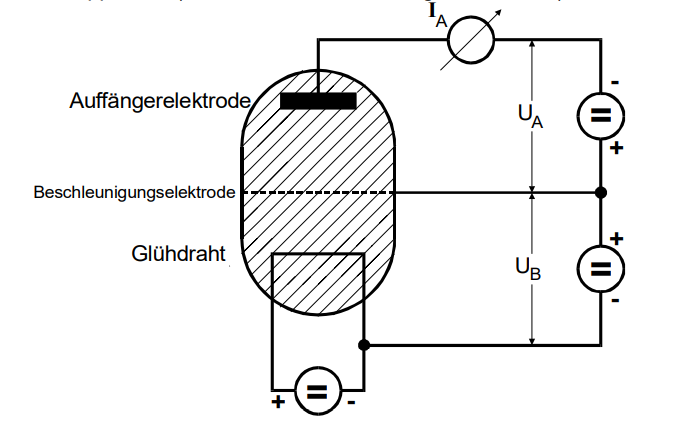
\includegraphics[scale=1]{content/PAufbau.png}
    \caption{Prinzipielle Aufbau des Frank-Hertz-Versuchs \cite{sample}.}
    \label{fig:FH}
\end{figure}

\begin{figure}[H]
    \centering
    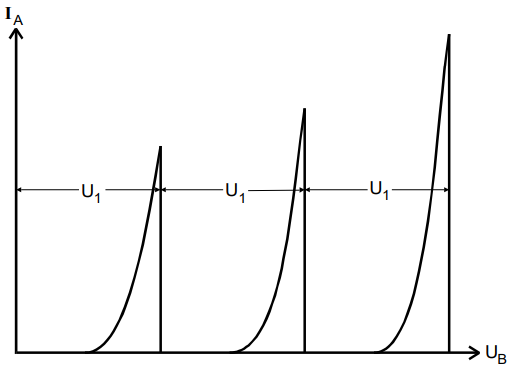
\includegraphics[scale=1]{content/Diskret.png}
    \caption{Idealisierter Zusammenhang zwischen Strom und Spannung \cite{sample}.}
    \label{fig:Diskret}
\end{figure}

\subsection{Einfluss des Kontaktpotentials}
\subsection{Einfluss des Energie-Spektrums der Elektronen}
\subsection{Einfluss des Dampfdruckes}
\subsection{Aufbau der Hg-Elektronenhülle}
\cite{sample}
